\documentclass[11pt]{article}

\usepackage{maiacustom}

\begin{document}

\psettitle{Banco de questões de astronomia}

Estas questões foram produzidas/selecionadas cuidadosamente com o objetivo de preparar os estudantes para o processo seletivo de astronomia no Brasil. Algumas questões não são de autoria própria e estão devidamente sinalizadas por () antes do enunciado. O template do banco de questões é o mesmo do Professor \text{Kevin Zhou}. Seu trabalho é valioso, e diversas ideias desta lista podem ser encontradas em seus Handouts.

% \begin{psidea}{Título da Ideia}{}
% Ideia
% \end{psidea}

% \begin{psexample}{Título do Exemplo}{}
% Exemplo
% \end{psexample}

% \begin{pssolution*}{}{}
% Solução
% \end{pssolution*}

% \begin{psremark*}{Título da Observação}{}
% Observação
% \end{psremark*} 
\section{Astronomia de Posição}

\pts{5} %problema da semana 114
\begin{pproblem} Após se perderem em uma navegação, você e o professor Klafke naufragam em uma ilha e encontram o seguinte relógio de Sol:
    \begin{figure}[H]
        \centering
        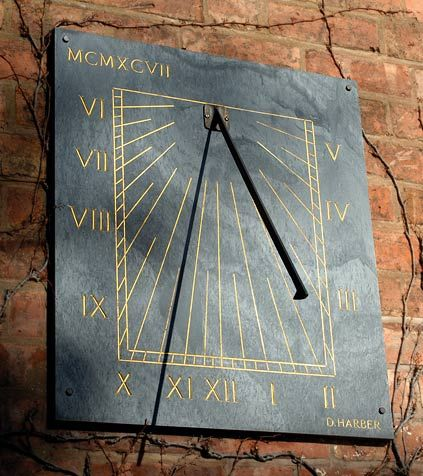
\includegraphics[width=0.5\linewidth]{imagens/q6.jpg}
        \caption{Relógio de Sol}
    \end{figure}
    Agora é missão de vocês descobrirem propriedades do relógio de Sol.
    \begin{enumerate}[label=\textbf{\alph*)}]
        \item Em qual hemisfério vocês se encontraram? Como você chegou a tal conclusão?
        \item Após várias semanas na ilha, vocês notam que a sombra do relógio parece seguir uma linha reta, sendo \(\phi\) a latitude que vocês se encontraram, determine a declinação do Sol nesse dia e explique o porquê disso só acontecer em \(2\) dias do ano.
        \item Prove que, quando o Sol possui a declinação encontrada anteriormente, a sombra segue uma linha reta. Isso pode ser feito seguindo os seguintes passos:
        \begin{enumerate}[label=\roman*)]
            \item Determine a orientação da linha e explique por que ela deve estar nessa orientação;
            \item Determine o comprimento da sombra para uma dada posição do Sol em coordenadas alt-azimute;
            \item Derive uma relação entre altitude e azimute, dado que a ponta da sombra está sobre a linha;
            \item Determine uma quantidade constante e mostre que ela é constante para todas as posições do Sol naquele dia.
        \end{enumerate}
    \end{enumerate}


\begin{pssolution*}{}{}
    \begin{alternativas}
        \item Pela imagem, podemos notar que as notações da esquerda correspondem às horas da manhã. Assim, temos que o Sol está nascendo à direita, para que assim a sua sombra fique sobre a esquerda. A partir desses argumentos, é possível dizer que o ponto cardeal \textit{Leste} se encontra à direita e o \textit{Oeste} à direita. Um relógio de sol vertical tem seu gnômon sempre apontado para o polo celeste não elevado. Como este está apontando para a direção \textit{Sul}, podemos concluir que o relógio se encontra no \(\boxed{\textit{hemisfério Norte}}\).

        \item Isso só acontece nos equinócios, quando \(\delta_\odot = 0\).

        \item Seguindo os passos do enunciado, 
        \begin{enumerate}[label=\roman*)]
            \item Como \(\delta_\odot=0\), o céu se move exatamente da direção leste para oeste, 
            \item Se o gnômon tem comprimento \(L\) e o Sol está em uma altura \(h\), utilizando geometria, podemos dizer que o comprimento da sombra, \(l\), vale, \(l=\frac{L}{\tan h}\).
            \item Observe a seguinte figura, 
            \begin{figure}[H]
                \centering
                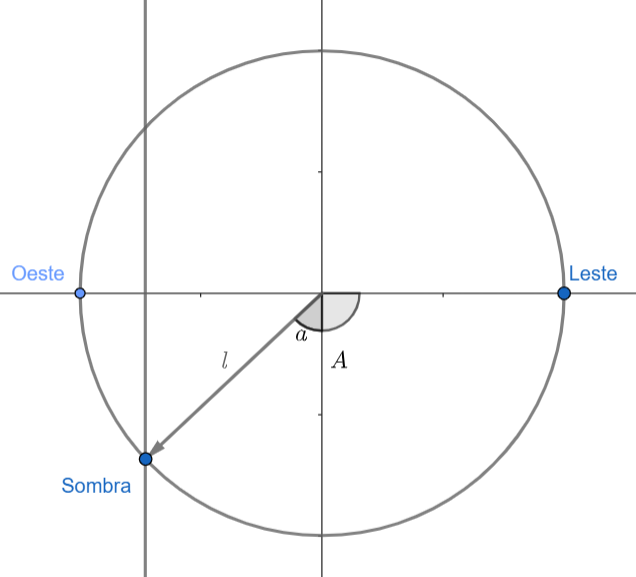
\includegraphics[width=0.66\linewidth]{imagens/retarelogiosolvert.png}
                \caption{Esquema da linha imaginária}
            \end{figure}
        \end{enumerate}

        A distância entre o centro do relógio e a sombra é dada por,

        \[x = l\sin (A-90^{\circ})\equiv l\sin a = L\frac{\sin a}{\tan h}\]

        Agora, queremos provar que essa quantidade é constante.

        \item Observe o seguinte triângulo: 
        
        \begin{figure}[H]
            \centering
            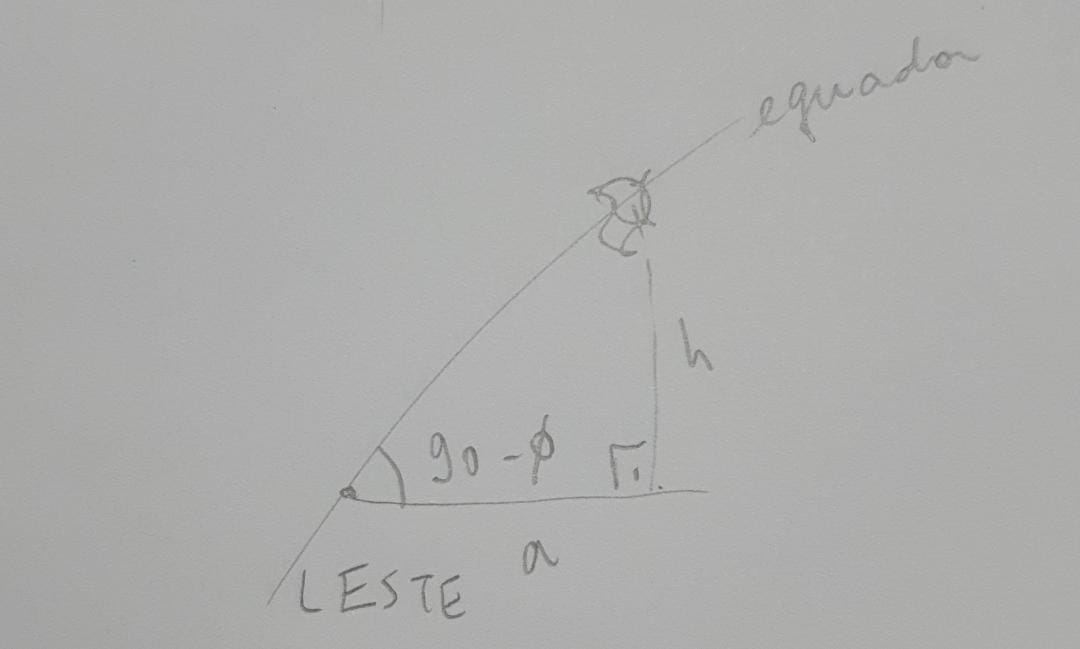
\includegraphics[width=0.5\linewidth]{imagens/trigesf1.jpg}
            \caption{Sol no equador}
        \end{figure}

        Usando a Lei dos quatro elementos, 

        \[\cot(90^\circ -\phi)\sin(90^{\circ})+\cos a \cos(90) = \cot h \sin a\]

        Simplificando, temos, 

        \[\frac{\sin a}{\tan h } = \tan {\phi}\]

        O que é constante. Logo, a nossa condição está provada.

    \end{alternativas}
\end{pssolution*}
\end{pproblem}

\pts{5}
\begin{pproblem} (Adaptado T1 - 2024)
    A equação do tempo é a diferença entre a ascensão reta do Sol médio e a ascensão reta do Sol verdadeiro. Sabendo disso, vamos calcular algumas de suas propriedades.
    \begin{alternativas}
        \item Determine uma expressão para a equação do tempo, desconsiderando a excentricidade da Terra, i.e.: O Sol possuindo velocidade constante ao longo da eclíptica. Deixe sua resposta em função do tempo desde o equinócio de março \(T_M\), do período da Terra \(T\) e da obliquidade da eclíptica \(\epsilon\).
        \item Agora, considerando a excentricidade da Terra, a equação do tempo tem forma:
        \[E.T. = -2e \cdot \sin(k_1 \cdot M) + \tan^2 \left( \frac{\epsilon}{2} \right) \cdot \sin\left( k_2 \cdot (M + \lambda_P) \right)\]
        Onde \(M\) é a anomalia média, \(\lambda_P\) a longitude eclíptica do periastro e \(e\) a excentricidade da Terra. Determine as constantes \(k_1\) e \(k_2\). Pense nas situações de simetria envolvendo cada uma das parcelas da equação.
        \\
        Agora o objetivo da questão é descobrir a declinação do Sol no ponto de nó do analema. Veja a figura a seguir:
        \begin{figure}[H]
            \centering
            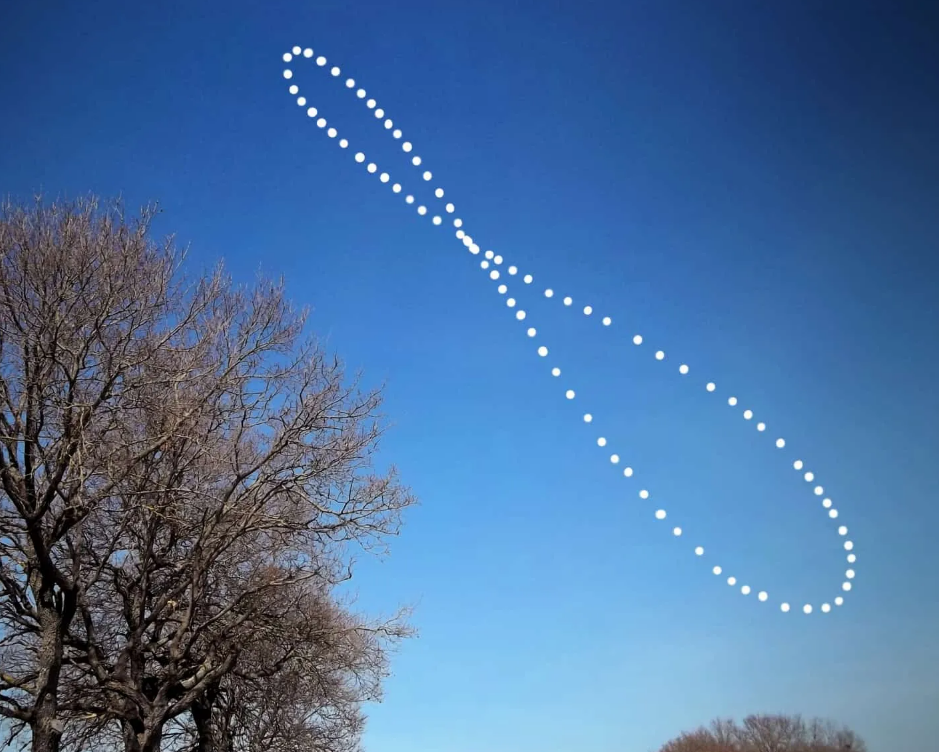
\includegraphics[width=0.7\textwidth]{imagens/q16.png}
            \caption{Representação analema}
        \end{figure}
        O ponto de nó é o ponto em que a trajetória se cruza.
        \item Para pequenos valores da declinação do Sol, obtenha uma fórmula para essa em função de \(M\), \(\lambda_P\) e \(\epsilon\). Considere também que a excentricidade e a inclinação da órbita sejam suficientemente pequenas.
        \item Encontre as duas anomalias médias que tenham a mesma declinação e mesma \(E.T.\).
        \item Encontre o valor da declinação solar no ponto de nó.
    \end{alternativas}

\begin{pssolution*}{}{ }
    \begin{alternativas}
        \item A equação do tempo se dá por
        
        \[E.T. = \alpha_M - \alpha_V\]

        Onde \(\alpha_M\) é a ascensão reta do Sol médio, i.e.: um "Sol fictício" que se move ao longo do equador com velocidade constante, e \(\alpha_V\) a ascensão reta do Sol verdadeiro.

        Observe o seguinte triângulo esférico

        COLOCAR imagem

        Primeiramente, tanto o Sol verdadeiro quanto o Sol médio possuem velocidades angulares constantes e equivalentes a \(\omega_\odot = 2\pi/T\), assim, \(\alpha_M=\omega_\odot T_M\).

        Utilizando a lei dos quatro elementos

        \[\cot \pi/2 \sin\epsilon + \cos\epsilon\cos\alpha_V=\cot(\omega_\odot T_M)\sin\alpha_V\]

        Como \(\cot\pi/2 =0\), obtemos

        \[\alpha_V = \tan^{-1}(\cos\epsilon\tan(\omega_\odot T_M))\]

        Note que, quando \(\epsilon = 0\), \(\alpha_V = \alpha_M\) como esperado.

        Por fim, voltando à definição da equação do tempo

        \[\boxed{E.T. = \tan^{-1}\left(\cos\epsilon\tan\left(\frac{2\pi}{T} T_M\right)\right) - \frac{2\pi}{T}T_M}\]

        \item Para resolver essa questão, vamos pensar nas situações de simetria. Para uma órbita elíptica, a única situação de simetria é em relação ao eixo maior. Já considerando a obliquidade da eclíptica, existem duas simetrias possíveis, em relação à linha dos solstícios e dos equinócios. Portanto, é razoável pensar que a senoide que se relaciona com a excentricidade da órbita tenha um período por ano, enquanto a que se relaciona com a obliquidade da eclíptica tenha 2 períodos por ano. Assim, \(\boxed{k_1=1, \ k_2 = 2}\)
        
        \item Voltando ao triângulo esférico anterior e utilizando a Lei dos Senos, nós temos
        
        \[\frac{\sin\delta_\odot}{\sin\epsilon} = \sin\lambda\]

        Onde \(\lambda \) é a longitude eclíptica do Sol. Utilizando que para pequenos ângulos \(\sin\theta \approx \theta\), temos

        \[\delta_\odot = \epsilon\sin\lambda\]

        Desprezando a excentricidade, temos \(\lambda = \lambda_P + M\), assim

        \[\boxed{\delta_\odot = \epsilon\sin(\lambda_P + M)}\]

        \item A condição para que duas anomalias médias possuam a mesma equação do tempo é 
        \[\sin(M_1+\lambda_P) = \sin(M_2+\lambda_P)\]

        Usando que \(\sin\theta = \sin(\pi-\theta)\) temos

        \[\boxed{M_2 =\pi -M_1-2\lambda_P}\]

        \item Igualando as equações do tempo
        
        \[-2e\sin(M_1) + \tan^2 \left( \frac{\epsilon}{2} \right)\sin\left(2(M_1 + \lambda_P) \right) = -2e\sin(M_2) + \tan^2 \left( \frac{\epsilon}{2} \right)\sin\left(2(M_2 + \lambda_P) \right)\]

        Substituindo \(M_2\)  

        \[-2e\sin(M_1) + \tan^2 \left( \frac{\epsilon}{2} \right)\sin\left(2(M_1 + \lambda_P) \right) = -2e\sin(M_1+2\lambda_P) - \tan^2 \left( \frac{\epsilon}{2} \right)\sin\left(2M_1 + 2\lambda_P \right)\]

        \[\tan^2 \left( \frac{\epsilon}{2} \right)\sin(2M_1+2\lambda_P) = e(\sin M_1 - \sin(M_1+\lambda_P))\]

        Utilizando o seno do arco duplo e prostaférese:

        \[\tan^2\left(\frac{\epsilon}{2}\right)\sin(M_1+\lambda_P)\cos(M_1+\lambda_P) = -e\sin\lambda_P\cos(M_1+\lambda_P)\]

        \[\sin(M_1+\lambda_P) = -\frac{e\sin\lambda_P}{\tan^2\left(\frac{\epsilon}{2}\right)}\approx -\frac{4e\sin\lambda_P}{\epsilon^2}\]

        Finalmente, substituindo na fórmula da declinação:

        \[\boxed{\delta_\odot \approx -\frac{4e\sin\lambda_P}{\epsilon}}\]
    \end{alternativas}
\end{pssolution*}
\end{pproblem}

    
\pts{5}
\begin{pproblem}
    Porílio, após um longo dia de aulas no ITA, durante solstício de verão (\(\phi = 23^\circ 11' S, \ \lambda = 45^\circ 53' O\)) deseja ver o por do Sol. No dia em questão, o valor da equação do tempo é \(E.T. = -3\) minutos. Porílio não quer perder o Sol de jeito nenhum e começa a correr para que o (centro do) Sol continue no horizonte.

    \begin{alternativas}
        \item São José dos Campos, segue o horário de Brasília (UTC-3h), em qual horário, no Tempo Civil, Porílio deve começar sua corrida?
        \item Se Porílio corre em direção a um dos polos geográficos, qual deve ser a sua velocidade inicial?
        \item Se Porílio decide subir uma montanha de inclinação \(i = 30^\circ\), a uma velocidade constante de \(v = 1\) m/s, qual o maior tempo com que Porílio consegue deixar o Sol acima do horizonte?
        \textbf{Dica: } Utilizar aproximações para pequenos ângulos, talvez seja útil.
    \end{alternativas}

\begin{pssolution*}{}{ }
    \begin{alternativas}
        \item Para encontrar o horário de nascer/por do Sol de uma estrela, precisamos achar o ângulo horário dela no momento em que ela nasce. Olhe o triângulo esférico a seguir, 
        
        \begin{figure}[H]
            \centering
            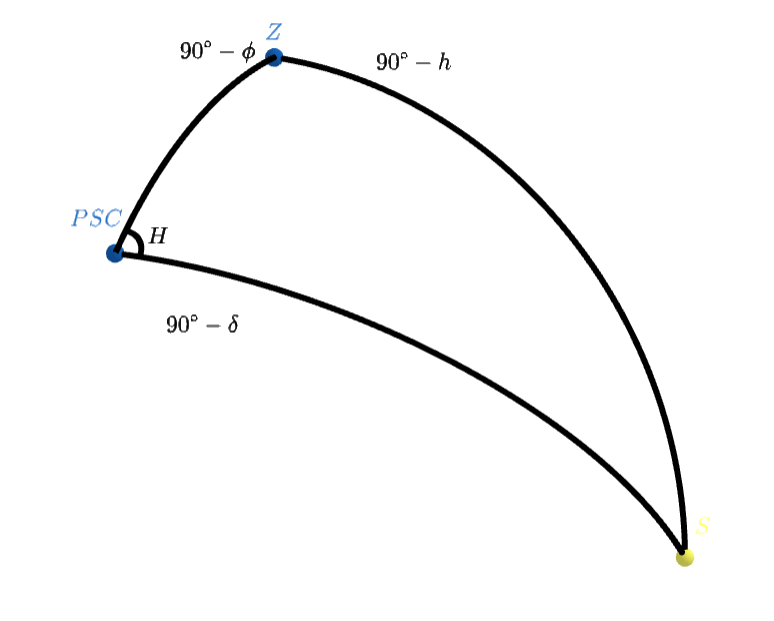
\includegraphics[width=0.8\linewidth]{imagens/trigangulohorario.png}
            \caption{Esquema do Sol no Horizonte}
        \end{figure}

        No momento em que o Sol se encontra no horizonte, temos \(h = 0\). Por ser o solstício de verão (no hemisfério Sul), temos \(\delta = -23^\circ 47'\). Utilizando a lei dos cossenos e que \(\sin(90 - \theta) = \cos(\theta)\) e que \(\cos(90 - \theta) = \sin(\theta)\), temos 

        \[\sin h = \sin\phi\sin\delta + \cos\phi\cos\delta\cos H\]

        Resolvendo para \(H\), e usando \(\sin h = \sin 0^\circ = 0\), 

        \[\cos H = -\tan\phi\tan\delta\]

        Resolvendo, obtemos \(H = 100,72^\circ = 6^h 42^m 52^s\)

        O horário do pôr do Sol é dado por \(TSL = 12 + H = 18^h 42^m 52^s\).

        Utilizando que \(TC = TSL + (\lambda_{\text{fuso}} - \lambda_{\text{local}})/15 - E.T.\), obtemos, 

        \[\boxed{TC = 18^h 49^m 20^s}\]

        \item Porílio deve correr em direção ao Polo Celeste Sul, uma vez que a declinação do Sol é negativa. Para achar sua velocidade inicial, vamos derivar a lei dos cossenos em relação ao tempo em \(h = 0\).
        \[\frac{d\cos H}{dt} = -\tan\delta \frac{d\tan\phi}{dt}\]

        Usando a regra da cadeia, 

        \[-\sin H \dot{H} = -\frac{\tan\delta}{\cos^2\phi}\dot{\phi}\]

        Onde \(\dot{a} = \frac{da}{dt}\). Isolando \(\dot{\phi}\), 

        \[\dot{\phi} = \frac{\cos^2\phi\sin H}{\tan\delta}\dot{H}\]

        A variação do ângulo horário é \(360^\circ / 24^h = 15^\circ / 1^h\). Resolvendo para \(\dot{\phi}\), 

        \[\dot{\phi} = -28,68^\circ/h = -1,39 \cdot 10^{-4} \text{ rad/s}\]

        Note que o sinal de \(\dot{\phi}\) apenas representa que ele está se movendo em direção ao polo Sul. Utilizando que, 

        \[\dot{\phi} = \frac{v}{R_\oplus}\]

        Chegamos na relação \(v = R_\oplus|\dot{\phi}|\),
        
        \[\boxed{v \approx 885 \text{ m/s}}\]

        \item Agora, temos que usar a ideia de ângulo do horizonte. Observe a seguinte imagem, 
            \begin{figure}[H]
                \centering
                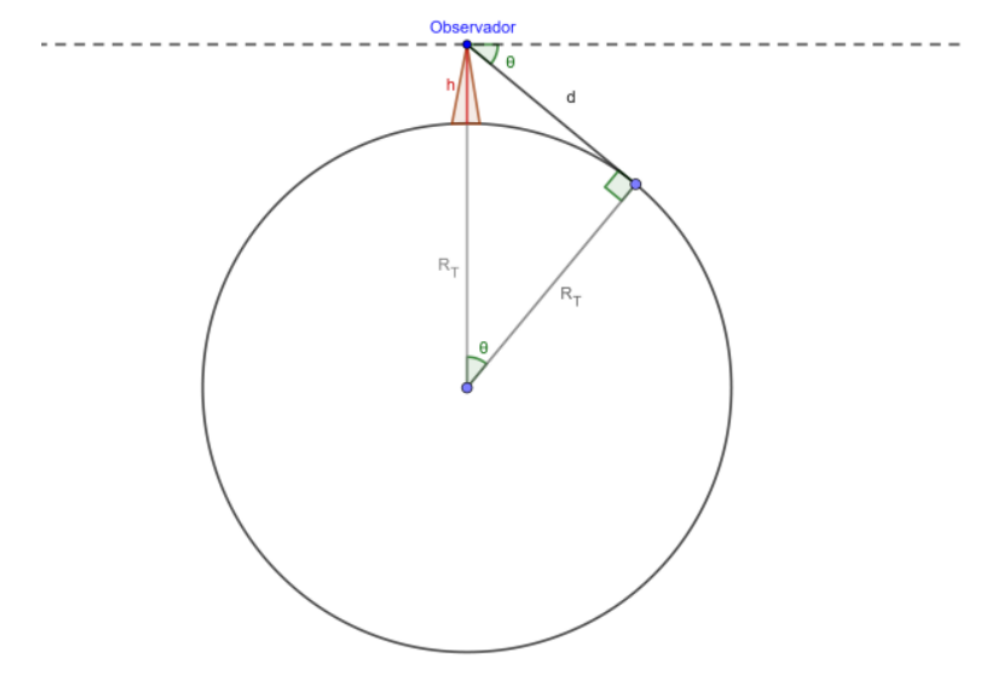
\includegraphics[width=0.90\linewidth]{imagens/angulohorizonte.png}
                \caption{Fonte: Apostila Magna}
            \end{figure}

            O ângulo \(\theta\) vale

            \[\cos\theta = \frac{R_T}{R_T + h}\]

            Como \(h \ll R_T\), vamos utilizar \(x = h / R_T\) e usar as aproximações para \(x \ll 1\).

            \[\cos\theta = \left(\frac{R_T + h}{R_T}\right)^{-1} = \left(1 + \frac{h}{R_T}\right)^{-1} \approx 1 - \frac{h}{R_T}\]

            Como \(\theta\) é um ângulo pequeno, vamos utilizar a aproximação em segunda ordem utilizando a série de Taylor, 

            \[f(x) \approx \sum \frac{f^{(n)}(a) x^n}{n!}\]

            Onde \(f^{(n)}(x)\) representa a n-ésima derivada de \(f(x)\). Expandindo a função em torno de \(a = 0\), temos, 

            \[\cos\theta \approx 1 - \frac{\theta^2}{2}\]

            Igualando os termos, 

            \[1 - \frac{\theta^2}{2} = 1 - \frac{h}{R_T} \rightarrow \theta = \sqrt{\frac{2h}{R_T}}\]

            Para calcular o tempo em que o Sol continua acima do horizonte, temos que calcular o tempo em que a altura aparente do Sol deve ser compensada pelo ângulo \(\theta\), a fim de que o Sol permaneça no horizonte. Desse modo, a lei dos cossenos se torna, 

            \[\sin\theta = \sin\phi\sin\delta + \cos\phi\cos\delta\cos H\]

            Usando \(\sin\theta \approx \theta\), 

            \[\theta = \sin\phi\sin\delta + \cos\phi\cos\delta\cos H\]

            Derivando os dois lados com relação ao tempo, (aqui vamos desprezar \(\dot{\phi}\) uma vez que a velocidade com que Porílio se move é muito pequena).

            \[\frac{d\theta}{dt} = -\cos\phi\cos\delta\sin H \dot{H}\]

            Para derivar \(\theta\) em relação ao tempo, perceba que \(h(t) = v t \sin i\).

            \[\frac{d\theta}{dt} = \sqrt{\frac{2v\sin i }{R_T}}\frac{d}{dt}\sqrt{t} = \sqrt{\frac{v\sin i}{2 R_T t}}\]

            Igualando as expressões, 

            \[\frac{v\sin i}{2R_T t} = (\cos\phi\cos\delta\sin H \dot{H})^2\]

            \[t = \frac{v\sin i}{2R_T(\cos\phi\cos\delta\sin H \dot{H})^2}\]

            \[\boxed{t \approx 10,82 \text{ s}}\]

    \end{alternativas}
    
\end{pssolution*}
\end{pproblem}



\pts{3}
\begin{pproblem}
    Mauí, um renomado astrônomo, deseja passar suas férias de fim de ano em Sergipe \((10^\circ \ 54'\ 33'' S, \ 37^\circ 4'29'' O\)) e deseja saber o horário de nascimento de uma de suas estrelas favoritas, All Kaf al Dij Ma \Romannum{3} \((\delta = +10^\circ \ 56'\ 58'', \ \alpha = 2h \ 58m \ 43s\)), e precisa de sua ajuda para calcular o horário de nascimento dela nas seguintes situações:
    
    \begin{alternativas}
        \item Calcule o horário de nascimento de All Kaf al Dij Ma \Romannum{3} no solstício de dezembro.
        \item Quanto tempo a estrela passará acima do horizonte?
        \item Estime o período de tempo em que a estrela é visível.
    \end{alternativas}

\begin{pssolution*}{}{ }
    \begin{alternativas}
        \item Como visto anteriormente, o ângulo horário de nascimento de uma estrela é calculado por: 

        \[\cos H = - \tan \delta \tan \phi \rightarrow H = \]

        O horário pode ser obtido usando a equação: 

        \[TSL = \alpha + H\]

        Resultando em \(\boxed{TSL = \text{resultado}}\)

        \item O tempo em que a estrela fica acima do horizonte é dado por: 
        
        \[\Delta t = 2 H = \]

        \item No solstício de verão, \(\delta_\odot = -23,47\), assim, o ângulo horário do sol é dado por, \(H_\odot = -\tan\delta_\odot \tan\phi = \), Ou seja, o tempo em que o Sol fica visível é dado por, \(\delta t_\odot = \). Uma estimativa válida do tempo em que a estrela é visível é dada por: 
        \[\Delta t = 2 (H - H_\odot)\]

        Que representam os períodos em que a estrela estará acima do horizonte sem a presença do Sol: 
       
        \[\boxed{\Delta t = \text{resultado}}\]
    \end{alternativas}
\end{pssolution*}
\end{pproblem}


\pts{4}
\begin{pproblem}(Lucas Cavalcante - \href{https://noic.com.br/olimpiadas/astronomia/problemas-da-semana/astronomia-semana-111/}{Semana 111})
    Considerando um sistema de coordenadas horizontal em que o azimute \(0\) corresponde ao ponto cardeal norte, um asteroide foi observado nas alturas \(h_1\) e \(h_2\) e azimutes \(A_1\) e \(A_2\), enquanto outro asteroide foi observado nas coordenadas \(h_3\), \(h_4\), \(A_3\) e \(A_4\). Encontre as coordenadas dos pontos de encontro entre os asteroides.
    
    \begin{psidea}{Notação de Einstein}{}
    Durante a resolução dessa questão, utilizarei a Notação de Einstein. Ela é uma ferramenta física para facilitar as contas vetoriais. Explicando, na notação comum, um vetor é representado por
    \[\mathbf{a} = (a_1 \hat{\mathbf{e}}_1, \ a_2 \hat{\mathbf{e}}_2, \ a_3 \hat{\mathbf{e}}_3)\]
    Na notação de Einstein, isso é substituído por:
    \[\mathbf{a} = a_i \hat{\mathbf{e}}_i\]
    Onde os índices repetidos indicam a soma (\(a_i \hat{\mathbf{e}}_i = a_1 \hat{\mathbf{e}}_1 + a_2 \hat{\mathbf{e}}_2 + a_3 \hat{\mathbf{e}}_3 + ...\))
    
    O produto escalar entre dois vetores, na notação de Einstein, é definido por:
    \[\mathbf{a}\cdot \mathbf{b} = a_i b_j \delta_{ij}\]
    Onde \(\delta_{ij}\) é a função \textit{Delta de Kronecker} e é definida por:
    \[\delta_{ij} = \left \{ \begin{matrix} 0, & \mbox{se } i \ne j \\ 
                                            1, & \mbox{se } i = j\end{matrix} \right.\]
    
    Assim, \(\mathbf{a}\cdot \mathbf{b} = a_i b_i \equiv a_1 b_1 + a_2 b_2 + a_3 b_3\)

    Já para o produto vetorial, temos:
        \[
        \mathbf{a} \times \mathbf{b} = a_i b_j \varepsilon_{ijk} \hat{\mathbf{e}}_k
        \]
        Aqui, \(\varepsilon_{ijk}\) é denominado \textit{tensor de Levi-Civita}, ou símbolo de Levi-Civita, e é definido como:
    
        \[
        \varepsilon_{ijk} = 
        \begin{cases} 
        +1 & \text{se } (i, j, k) \text{ é uma permutação par de } (1, 2, 3), \\
        -1 & \text{se } (i, j, k) \text{ é uma permutação ímpar de } (1, 2, 3), \\
        0 & \text{se dois ou mais índices são iguais}.
        \end{cases}
        \]

        Por exemplo, \(\varepsilon_{123} = \varepsilon_{312} = \varepsilon_{231} = 1\) e \(\varepsilon_{132} = \varepsilon_{213} = \varepsilon_{321} = -1\).
        Explicitamente 
        \[\mathbf{a} \times \mathbf{b} = (a_2 b_3 - a_3 b_2) \hat{\mathbf{e}}_1 + (a_3 b_1 - a_1 b_3) \hat{\mathbf{e}}_2 + (a_1 b_2 - a_2 b_1) \hat{\mathbf{e}}_3\]
   
        Também é de extrema importância a identidade 

        \[\varepsilon_{a,b,c}\varepsilon_{a,d,e} = \delta_{b,d}\delta_{c,e}-\delta_{b,e}\delta_{c,d}\]
    \end{psidea}
\begin{pssolution*}{}{}
    Para resolver esse problema, vamos utilizar dois conceitos importantíssimos de vetores. Sendo dois vetores $\mathbf A$ e $\mathbf B$. É dado que, $\mathbf A \cdot \mathbf B$ faz parte do plano formado pelos vetores $\mathbf A$ e $\mathbf B$, já $\mathbf A \times \mathbf B$ é perpendicular a esse plano. Assim, seja $\mathbf r_1$ e $\mathbf r_2$ dois vetores representando as posições do primeriro asteroide e $\mathbf r_3$ e $\mathbf r_4$ os dois vetores posições do segundo asteroide. A orbita do primeiro asteroide está contida no plano de $\mathbf r_1 \cdot \mathbf r_2$ e a órbita do segundo asteróide está contida no plano $\mathbf r_3 \cdot \mathbf r_4$. Mas, o que é interessante para resolver essa questão é analizar o produto vetorial, pois esse é perpendicular a órbita. Para melhor visualização, vamos olhar a seguinte imagem:

    \begin{figure}[H]
        \centering
        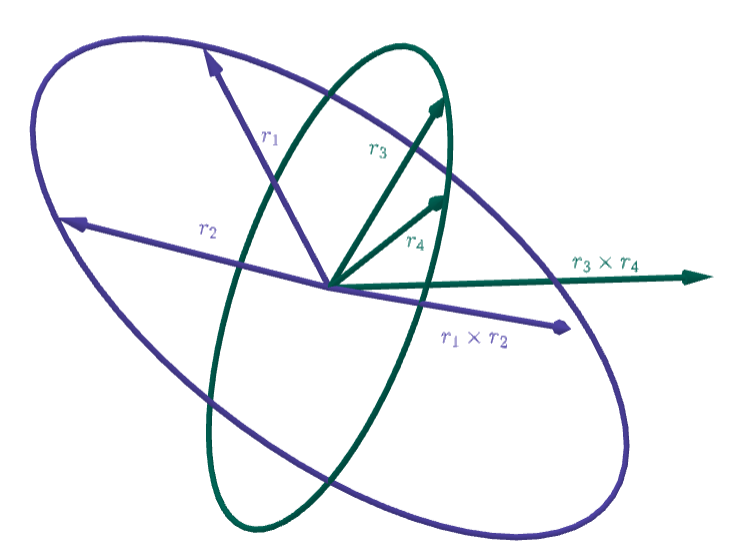
\includegraphics[width=0.8\linewidth]{imagens/orbitas3.png}
        \caption{Esquema das órbitas e visualização das multiplicações vetoriais}
    \end{figure}

    Agora, quando vamos além e fazemos a operação \((\mathbf r_1 \times \mathbf r_2)\times(\mathbf r_3 \times \mathbf r_4)\) temos um vetor que é perpendicular tanto ao vetor \(\mathbf r_1\times \mathbf r_2\) e quando o vetor \(\mathbf r_3\times \mathbf r_4\). E esse vetor, \textbf{necessariamente} passa pelo ponto comum entre as órbitas.

    \begin{figure}[H]
        \centering
        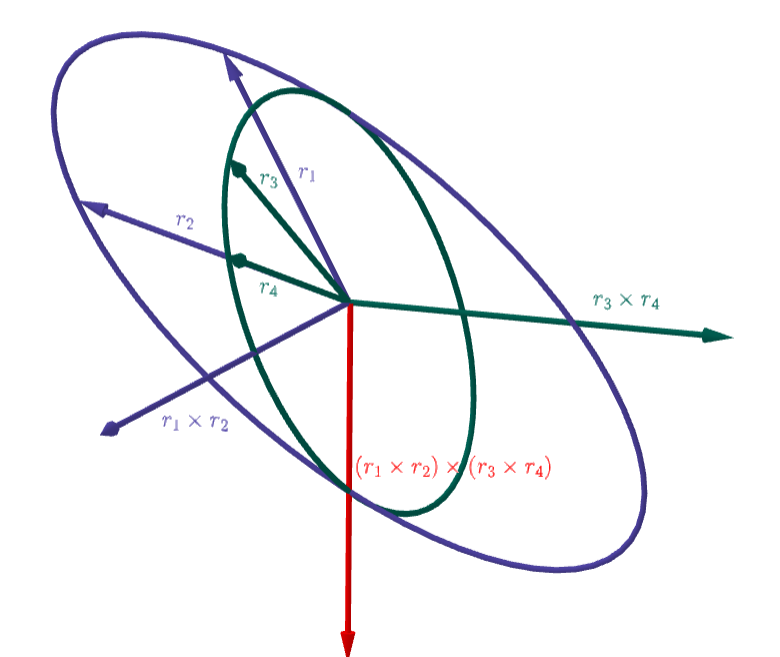
\includegraphics[width=0.8\linewidth]{imagens/orbitas4.png}
        \caption{Ponto de encontro}
    \end{figure}

    Note que pela simetria $(\mathbf r_3\times \mathbf r_4)\times(\mathbf r_1\times \mathbf r_2)\equiv - (\mathbf r_1 \times \mathbf r_2)\times (\mathbf r_3 \times \mathbf r_4)$ também será um ponto de encontro. Agora, vamos calcular esse vetor.

    Para conventer o vetor definido por $h_i$ e $A_i$ (em coordenadas esféricas) para $x_i$, $y_i$ e $z_i$ temos o seguinte, 

    $$\mathbf r_i = (\cos h_i\cos A_i, \ \cos h_i\sin A_i, \ \sin h_i)$$

    Aonde orientamos nossos eixos do modo que $x$ aponta para o norte e $z$ para o zênite. Indo para o cálculo e usando a notação de Einsten, 

    \[(\mathbf r_1 \times \mathbf r_2)\times(\mathbf r_3 \times \mathbf r_4) = (r_{1,i}r_{2,j}\varepsilon_{i,j,k}\mathbf{\hat{e}}_k)\times(r_{3,m}r_{4,n}\varepsilon_{m,n,o}\mathbf{\hat{e}}_o)\]

    Simplificando, 

    \[= \varepsilon_{i,j,k}\varepsilon_{m,n,o}r_{1,i}r_{2,j}r_{3,m}r_{4,n}(\varepsilon_{k,o,p}\mathbf{\hat{e}}_p)\]
    \[= \varepsilon_{i,j,k}\varepsilon_{m,n,o}\varepsilon_{k,o,p}r_{1,i}r_{2,j}r_{3,m}r_{4,n}\mathbf{\hat{e}}_p\]

    Agora para simplificar, vamos usar a identidade 

    \[\varepsilon_{a,b,c}\varepsilon_{a,d,e} = \delta_{b,d}\delta_{c,e}-\delta_{b,e}\delta_{c,d}\]

    Dessa maneira, nossa expressão se torna, 

    \[\varepsilon_{m,n,o}r_{3,m}r_{4,n}(\delta_{io}\delta_{jp}-\delta_{ip}\delta_{jo})r_{1,i}r_{2,j}\mathbf{\hat e}_p\]
    
    Resolvendo as deltas de Kronecker, nossa expressão se resume para, 

    \[(\varepsilon_{m,n,o}r_{3,m}r_{4,n}r_{1,o}r_{2,p}-\varepsilon_{m,n,o}r_{3,m}r_{4,n}r_{1,p}r_{2,o})\mathbf{\hat e}_p\]

    A primeira vista, isso pode parecer assustador ou até mais complicado que a expressão vetorial, mas com a prática da notação, a leitura se torna mais flúida e objetiva. Com um trabalho de corno, chegamos em, 

    \[\boxed{(\mathbf r_1 \times \mathbf r_2)\times(\mathbf r_3 \times \mathbf r_4) = T_1\mathbf r_2 - T+2\mathbf r_1}\]

    Onde

    \[
    \begin{aligned}
    T_1 &= 
    \cos h_1 \cos h_3 \sin h_4 \sin(A_3 - A_1)
    + \cos h_1 \cos h_4 \sin h_3 \sin(A_1 - A_4) \\
    &\quad + \sin h_1 \cos h_3 \cos h_4 \sin(A_4 - A_3)
    \end{aligned}
    \]

    \[
    \begin{aligned}
    T_2 &=
    \cos h_2 \cos h_3 \sin h_4 \sin(A_3 - A_2)
    + \cos h_2 \cos h_4 \sin h_3 \sin(A_2 - A_4) \\
    &\quad + \sin h_2 \cos h_3 \cos h_4 \sin(A_4 - A_3)
    \end{aligned}
    \]

    Embora interessante, cehgar numa fórmula fechada é muito trabalhoso, porém esse tipo de abordagem é ideal para trabalhar com valores númericos, torando problemas díficeis em versões muito mais simplistas.
\end{pssolution*}
\end{pproblem}


\pts{5}
\begin{pproblem} (Lista \(1\) - Vinhedo 2024) Considere um relógio de Sol composto por um mostrador vertical
    e um gnômon, conforme mostrado na figura.
    \begin{figure}[H]
        \centering
        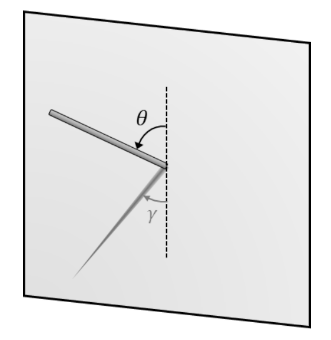
\includegraphics{imagens/q20.png}
        \caption{Esquema relógio de Sol.}
    \end{figure}
    \begin{alternativas}
        \item Suponha um relógio de Sol vertical cujo gnômon esteja corretamente apontado para o sul.
        Seja \(\phi\) a latitude do observador, \(H\) o ângulo horário do Sol e \(\delta\) a declinação solar. Determine
        a relação entre \(\theta\) e \(\gamma\) em função dessas variáveis.
        
        \item Com base no item anterior, qual deve ser o valor de \(\theta\) para que o relógio funcione durante o ano todo?

        \item Utilizando o valor correto para \(\theta\), determine a relação entre \(\gamma\) e \(H\), em função de \(\phi\) apenas.
    \end{alternativas}
\end{pproblem}

\pts{2} 
\begin{pproblem}
    Qual a menor altura que um gigante (que vive MUITOS), localizado no polo Sul, precisa ter para conseguir ver todas as estrelas do céu?

    \begin{pssolution*}
        O ângulo abaixo do horizonte que o gigante consegue enxergar é dado por: 
    
        \[\cos\theta = \frac{R_\oplus}{R_\oplus + H}\]
    
        Onde \(H\) é a altura do gigante. Devido à precessão dos equinócios, o polo sul ficará a \(23,47^\circ\) acima da eclíptica. Logo, o ângulo do horizonte deve ser \(\theta = 90^\circ - 23,47^\circ = 66,53^\circ\). Resolvendo para \(H\), temos:
    
        \[\boxed{H = R_\oplus\left(\frac{1}{\cos\theta}-1\right) \approx 9,62\cdot 10^6\text{ m}}\]
    \end{pssolution*}
\end{pproblem}    


\pts{3}
\begin{pproblem}
    Toleduardo deseja ver o pôr do Sol, mas acabou passando tempo demais na SorveterITA. Toleduardo é um homem \textit{Just in time} e deseja saber quanto tempo o pôr do Sol vai durar, para que ele possa se atrasar com calma. Sabendo que Toleduardo só vai para a SorveterITA nos dias 21 de março ou 22 de setembro, calcule qual é a duração do pôr do Sol na SorveterITA.
    \\
    \textbf{Dados: } Latitude da SorveterITA \(\phi = 23^\circ \ 10' \ 45''S, \ \ \lambda = 45^\circ 53' 14''O\).
\end{pproblem}
\begin{pssolution*}{}{}
    
    Para resolver essa solução, vamos invocar o triângulo de posição para o Sol, equacionando para o seu angulo horário.

    \[\sin h = \sin\delta\sin\phi + \cos\delta\cos\phi\cos H\] 

    Derivando em relação ao tempo, 

    \[\dot h \cos h = -\dot H \cos\delta\cos\phi \sin H\]

    No por do sol, 

    \[H_0 = \cos^{-1}\left(-\tan\delta\tan\phi\right)\]

    Nas próximidades de \(h=0\), temos, 

    \[\left. \frac{dh}{dt}\right|_{h=0} = -\dot H \cos\delta\cos\phi\sin H_0\]

    No dia em questão, \(\delta = 0\) (equinócios), logo \(H_0 = 6h\)

    \[\left. \frac{dh}{dt}\right|_{h=0} - \dot{H}\cos\phi\sin H_0\]

    Note que \(\dot H = 15^{\circ}/h\). Resolvendo para \(dt\), 
    
    \[dt \approx \frac{-dh}{\dot{H}\cos\phi \sin H_0}\]

    Integrando e usando que \(\sin H_0 = 1 \), 

    \[\Delta t \approx -\frac{1}{\dot H \cos \phi}\int_{\theta\odot}^{-\theta\odot}dh\]

    \[\Delta t \approx \frac{2\theta_\odot}{\dot H \cos \phi}\]

    \[\boxed{\Delta t \approx 4^m38^s}\]
\end{pssolution*}


\pts{3}
\begin{pproblem} (Lista 2 - Vinhedo 2021)
    Em fevereiro de 2015, a Lua iniciou um ciclo de ocultações mensais de Aldebaran ($\alpha$ Tau). Ou seja, todo mês a Lua passava na frente de Aldebaran para um observador na Terra. Vale ressaltar que essas ocultações não ocorriam necessariamente para observadores na mesma posição todo mês. 

    Calcule a data (mês e ano) do fim desse ciclo de ocultações mensais. Considere que a órbita da Lua é circular.

    \subsection*{Dados:}

    \begin{itemize}
        \item Latitude eclíptica de Aldebaran = $5,47^\circ$
        \item Período de precessão nodal da Lua = 18,6 anos
    \end{itemize}
\end{pproblem}


\pts{4}
\begin{pproblem} (Lista 2 - Vinhedo 2021)
    Miguel vive em uma ilha isolada no Oceano Pacífico Sul, em uma longitude
    $\lambda = 176^{\circ}09^{\prime}137,7^{\prime\prime}\text{W}$. Ao longo do ano, o local onde o Sol nasce, visto por Miguel, varia $\Delta A = 67^{\circ}03^{\prime}81^{\prime\prime}$ no horizonte. Para os dois primeiros itens, desconsidere a refração atmosférica. Com essas informações, descubra:

    \begin{alternativas}
        \item A latitude $\phi$ e o nome da ilha. (Consulte o Google Earth ou software similar)
        \item O intervalo de horários em que o Sol nasce na ilha, dado o fuso horário peculiar $UT + 12\frac{3}{4}$.
        \item Considerando a refração atmosférica, o tamanho do intervalo do item anterior iria diminuir, aumentar ou se manter constante?
    \end{alternativas}

\end{pproblem}


\pts{3}
\begin{pproblem}(Lista 2 - Vinhedo 2022) 
    Bruno decidiu alugar uma casa para passar as férias em Cuiabá ($15,3^{\circ} \text{S}$, $56,1^{\circ} \text{O}$). Como um bom astrônomo, Bruno passava suas noites sentado em uma cadeira observando as estrelas por uma porta gigante voltada para o ponto cardeal sul.

    A porta tinha 4,00 metros de altura e 1,50 metros de largura. Bruno tinha o costume de sentar a
    1,00 metro da porta perfeitamente alinhado com o seu centro na horizontal. Ou seja, o segmento
    de reta entre os olhos de Bruno e o ponto que está exatamente no meio da porta na horizontal e
    na altura dos olhos forma um ângulo de $90^{\circ}$ com o plano da porta. Os olhos de Bruno ficam a
    1,20 metros do chão quando ele está sentado na cadeira.
    
    Para facilitar as suas observações, Bruno criou um sistema de coordenadas baseado na posição da
    porta, de onde ele via as estrelas a partir do local onde estava sentado, utilizando metros como
    a unidade de referência. A origem do sistema está localizada no canto inferior esquerdo. As coordenadas
    em $x$ aumentam para a direita e as coordenadas em $y$ aumentam para cima. Dessa forma, uma
    estrela vista a 1 metro do lado esquerdo da porta e 2 metros acima do chão seria representada
    pelas coordenadas $(1, 2)$.
    
    Bruno estava bastante interessado em Shaula ($\lambda \ \text{Sco}, \delta = 37,1^{\circ} \text{S}$). Determine as coordenadas de
    Shaula no instante em que a estrela se tornava visível para Bruno quando observada através da porta. Assuma que Shaula estava abaixo do horizonte quando Bruno começava a observar o céu.
    
\end{pproblem}

\end{document}